\documentclass[12pt, a4paper]{article}  
\usepackage{amsmath,amsfonts,amssymb,amsthm,mathtools}  % пакеты для математики
\usepackage{fontspec}         % пакет для подгрузки шрифтов
\setmainfont{Roboto}       % задаёт основной шрифт документа

\usepackage{unicode-math}     % пакет для установки математического шрифта
\setmathfont{Asana Math}      % шрифт для математики

\usepackage{polyglossia}      % Пакет, который позволяет подгружать русские буквы
\setdefaultlanguage{russian}  % Основной язык документа
\setotherlanguage{english}    % Второстепенный язык документа
\usepackage{graphicx}
\graphicspath{}
\DeclareGraphicsExtensions{.pdf,.png,.jpeg,.jpg}

\author{Лищук Диана}
\title{Домашняя работа}
\date{11/02/2017}

\begin{document}

\maketitle 
%Написать в нём перечень с 10 фактами о себе

\section{Факты о себе}
\begin{enumerate}
\item Меня зовут Диана Лищук
\item Я родилась в городе Томск
\item Училась в музыкальной школе
\item Люблю смотреть сериалы, фильмы, периодичестки читать книги и посещать музей и выставки
\item Боюсь всяких насекомых, кроме бабочек и стрекоз
\item Любимое домашнее животное - кот
\item Хожу на фитнес
\item Обожаю гулять по ночному городу
\item Люблю путешествовать в разные страны
\item Учусь В РАНХиГС на отделении экономики =(
\end{enumerate}
 %Вставить свою фотографию
 
 \section{Фото}
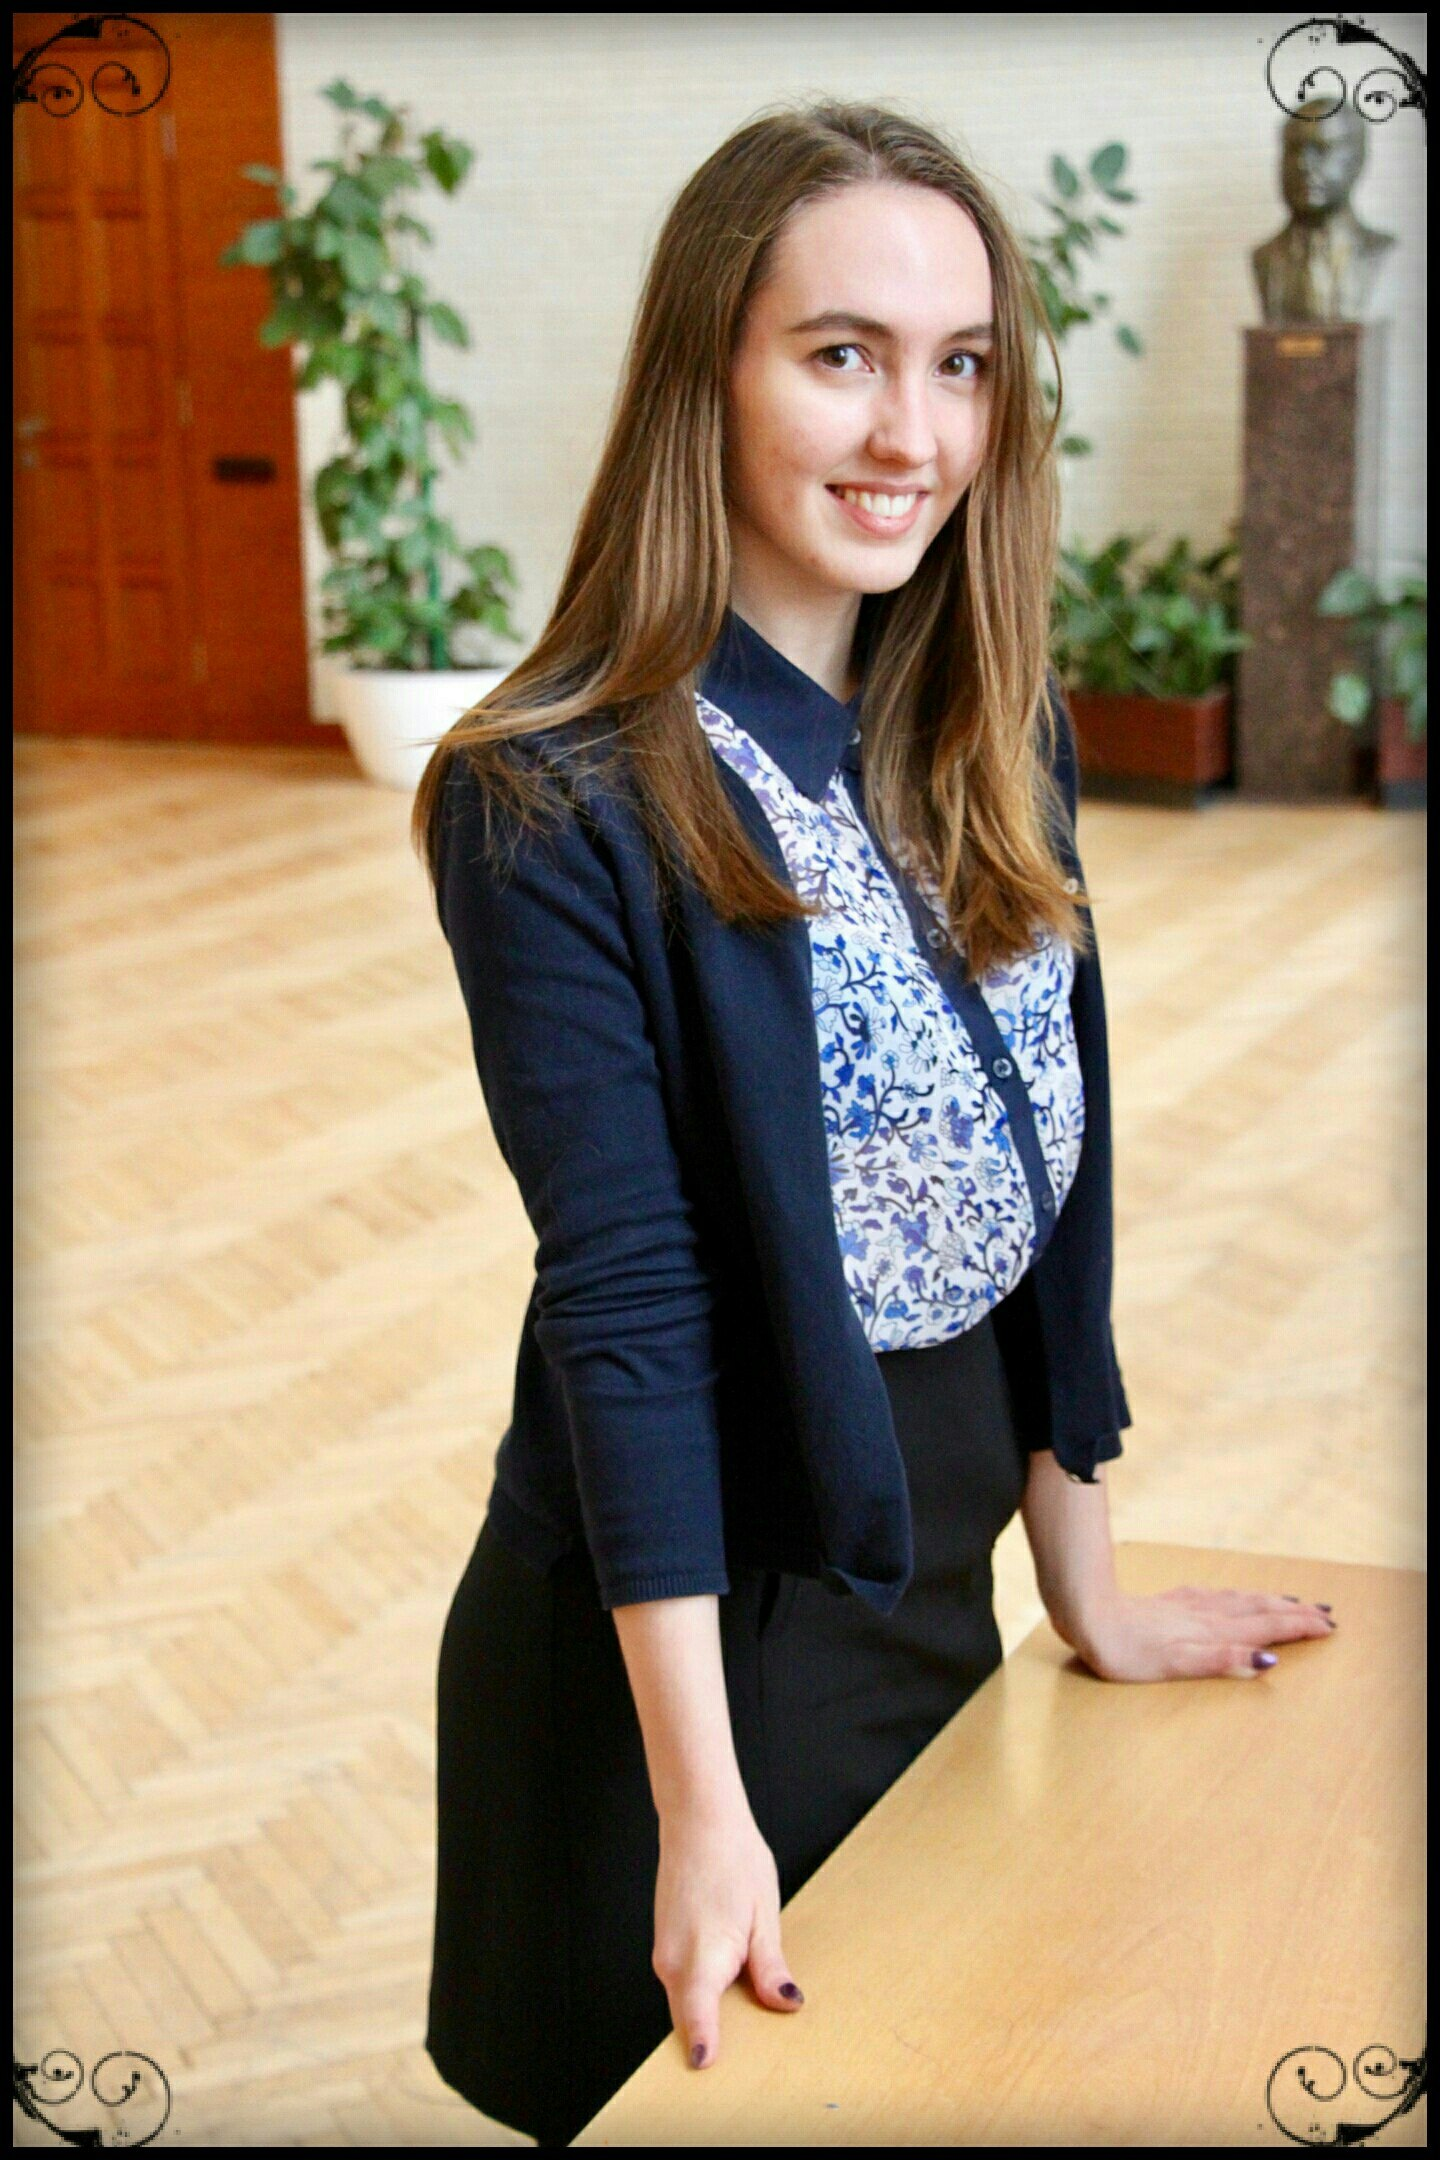
\includegraphics[scale=0.05]{8i3thmz0UAI}
%width=xx	Задаёт ширину рисунка равной xx
%heigth=xx	Задаёт высоту рисунка равной xx (если задана только ширина или только высота, то рисунок масштабируется пропорционально)
%scale=xx	Умножает размеры изображения на коэффициент xx
%angle=xx	Поворачивает изображение на xx градусов по часовой стрелке

%Написать 5 своих любимых сложных формул и одну ненавистную
\section{Формулы}
\subsection{Любимые формулы}
\begin{enumerate}
\item Формула суммы для убывающей геометрической прогрессии:\[ S_n = \sum_{i=1}^{n} \frac{b_1(1-q^n)}{1 - q} \tag{æ}\label{aster 1} \]
\item Свойства определённого интеграла: \[ \int_a^b (f_1(x)+f_2(x))dx = \int_a^b f_1(x)dx + \int_a^b f_2(x)dx \tag{æ æ}\label{aster 2} \]
\item Матричная форма множественной регресcии: \[ 
\def \Y {\begin{pmatrix} Y_1 \\ Y_2 \\ \vdots \\ Y_n \end{pmatrix}} 
\def \X' {
\begin{pmatrix} 
1 & X_{1,1} & \cdots & X_{k,1} \\
1 & X_{1,2} & \cdots & X_{k,2} \\
\vdots & \vdots & \ddots & \vdots \\
1 & X_{1,n} & \cdots & X_{k,n} \\
\end{pmatrix}}
\def \U {\begin{pmatrix} U_1 \\ U_2 \\ \vdots \\ U_n \end{pmatrix}}
\def \b {\beta}
\def \B {\begin{pmatrix} \b_0 \\ \b_1 \\ \vdots \\ \b_k \end{pmatrix}}
\Y=\X' \B + \U \tag{æ æ æ}\label{aster 3} \]
\item \[\textstyle\lim\limits_{n \to \infty} \left(\frac{1}{n+1} + \frac{1}{n+2} + \cdots + \frac{1}{2n}\right) = \ln2 \tag{æ æ æ æ}\label{aster 4} \]
\item Формула МНК-оценки для $\beta_1$ в модели парной регрессии: \[ \hat{\beta}_1 = \frac{\sum\limits_{i=1}^{n} (X_i-\overline{X})(Y_i-\overline{Y}) }{\sum\limits_{i=1}^{n} (X_i-\overline{X})^2} \tag{æ æ æ æ æ}\label{aster 5} \] 
\end{enumerate}

\subsection{Нелюбимая формула}
Ряд Тейлора: \begin{multline}  \sum_{k=1}^{\infty} \frac{f^{(k)}(a)}{k!} (x-a)^k = f(a) + \frac{f'(a)}{1!} (x-a)+ \frac{f"(a)}{2!} (x-a)^2 + \cdots + \\ +\frac{f^{(n)}(a)}{n!} (x-a)^n+ \cdots \tag{æ æ æ æ æ æ}\label{aster 6} \end{multline}

%Рассказать почему ты любишь какие-то формулы, а какие-то нет
\subsection{Объяснение}
Формула \eqref{aster 1} нравится, т.к. часто помогала искать пределы \\
Формула \ref{aster 2} логична \\
Формула \ref{aster 3} удобная вещь в метрике \\
Формула \ref{aster 4} просто понравилась \\
Формула \ref{aster 5} - это то единственное в метрике, что я могу посчитать \\
Формула \ref{aster 6} попалась мне на экзамене по мат. анализу. Принимал Попов 
\includegraphics[scale=0.05]{cep}


\end{document}

